\section{Nicolas Galland / Maxime Jacque (CESI - Sept$11^{th}$ - Oct $11^{th}$ 2017)}

Nicolas Galland and Maxime Jacque are working at the LF2L in the framework of "Introduction to the research" module.
The time is September 11 to October 11

\subsection{Context of their mision}

The context of the project is the extrusion process at LF2L (figure \ref{Context.Nicolas.Maxime})

\begin{figure}[H]
	\centering
	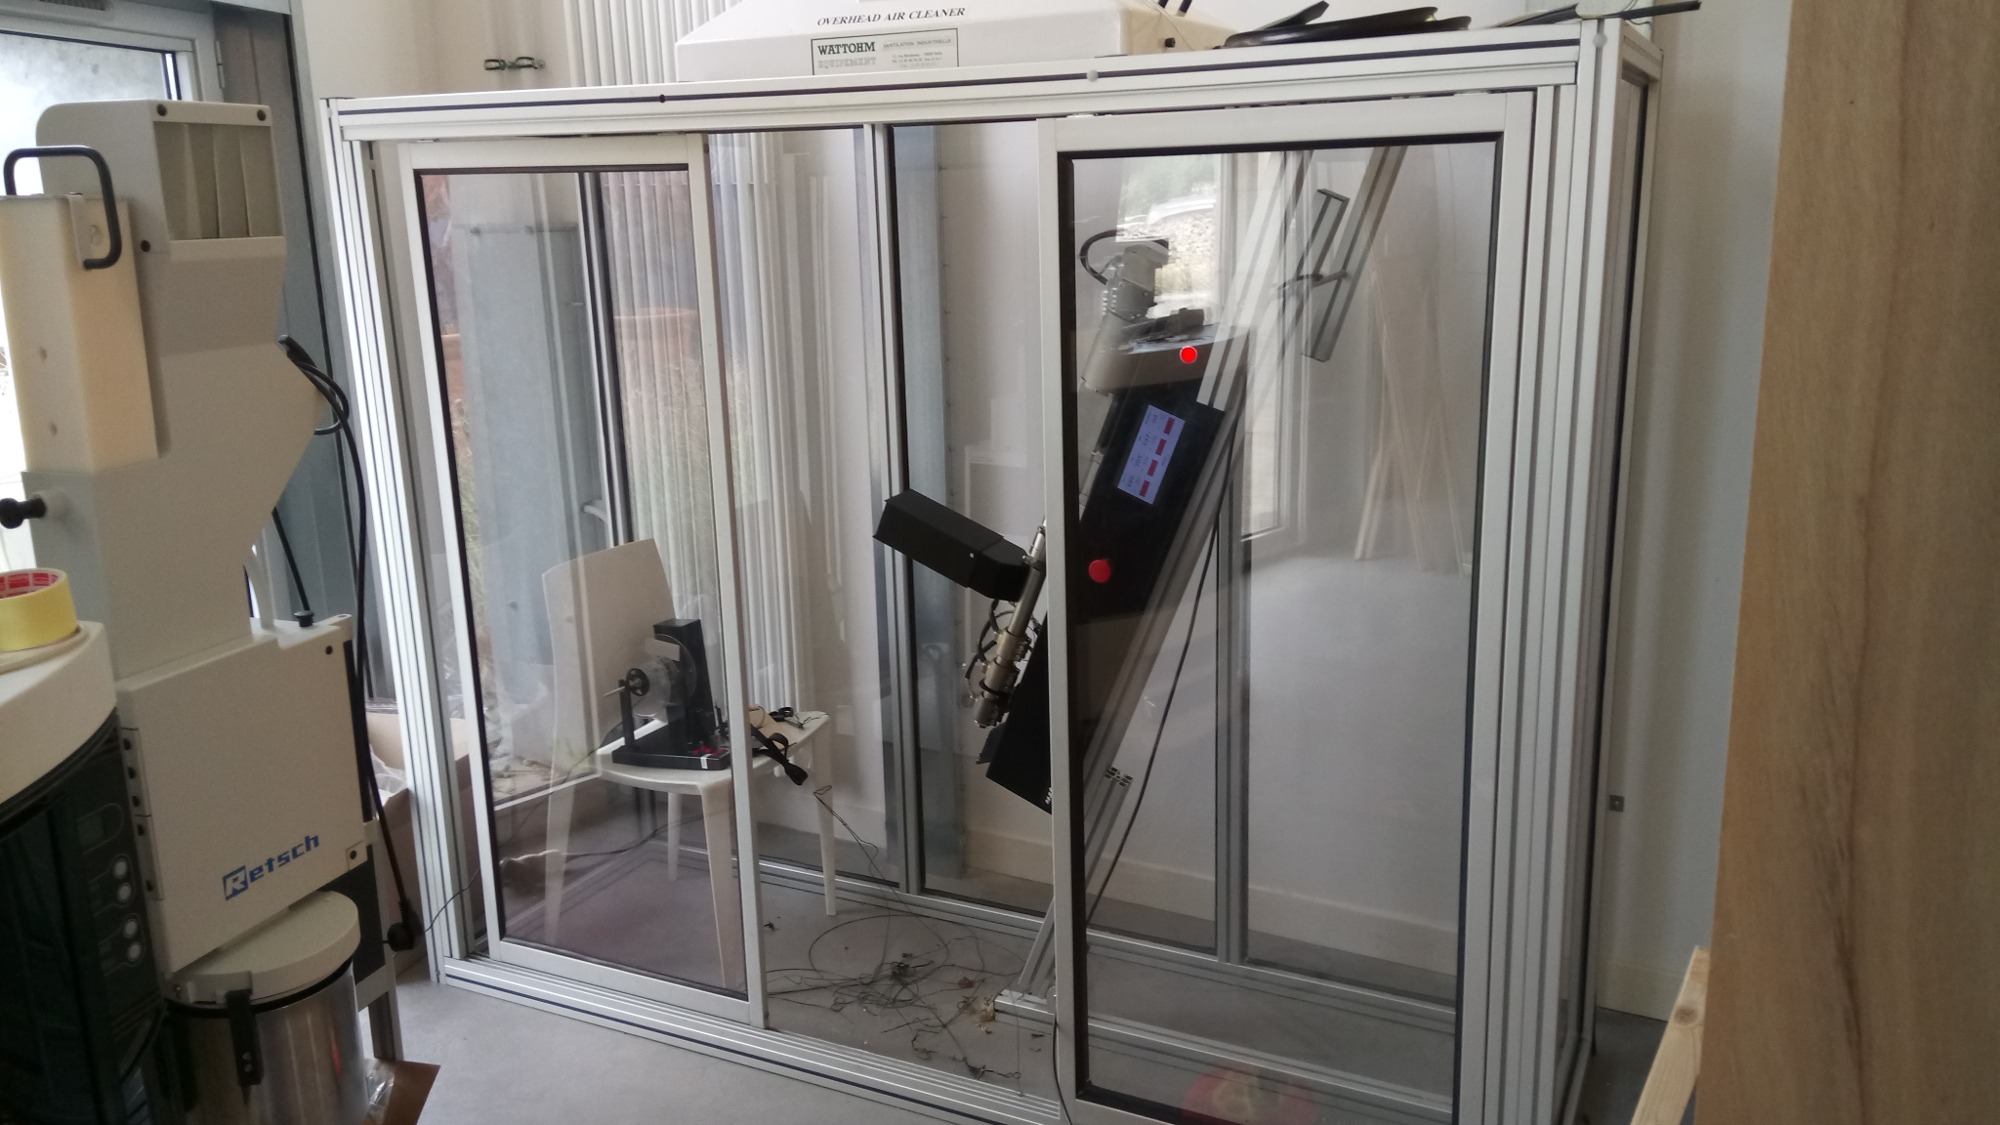
\includegraphics[width=0.7\textwidth]{Figures/Extrusion/Extruder.jpg}
	\caption{Extrusion process at Lorraine Fab Livin Lab}
	\label{Context.Nicolas.Maxime}
\end{figure}


\subsection{Objectives of the project}


The goal of the stage is to define and testing a functional prototype for feeding process in the extrusion machine at LF2L.




\begin{itemize}
	\item Exploration of concepts
	\item Definition of the operational conditions
\end{itemize}


Elements to consider:

\begin{itemize}
	\item State of the Art about Quality in 3D printing.
	\item Grey literature of 3D printing. 
\end{itemize}


\subsection{Expected elements to the end of the project}

The following elements are expected as results:

\begin{itemize}
	\item Tutorial to use the prototype
	\item Functional prototype
	\item Poster (Infography)  about the printing process at LF2L.
\end{itemize}


\newpage
\begin{landscape}
	
	\thispagestyle{empty}
	
	\subsection{Plannig September $11^{th}$ - October $11^{th}$ 2017}
	
	
\begin{adjustbox}{width={\linewidth}, keepaspectratio }


	
	\begin{gantt}{20}{25}
				
		\begin{ganttitle}
			\titleelement{Week -1}{5}
			\titleelement{Week - 2}{5}
			\titleelement{Week - 3}{5}
			\titleelement{Week - 4}{5}
			\titleelement{Week - 5}{5}
		\end{ganttitle}
		
		
		
		\begin{ganttitle}
			\numtitle{1}{1}{25}{1}
		\end{ganttitle}
		
		%	Week 1
		\ganttgroup{\textbf{Introduction to 3DP }}{0}{5}
		\ganttbar{Introduction to the project}{0}{2}
		\ganttbar{Literature of 3DP and Extrusion}{2}{4}
		% Goal of the Week
		\ganttmilestonecon[color=cyan]{\textcolor{ForestGreen}{Students know the project!}}{5}


		%	Week 2		
		\ganttgroup{\textbf{Literature review:}}{5}{5}
		\ganttbar{Extrusion process}{5}{2}
		\ganttbar{Experimental trials}{6}{2}
		\ganttbar{Exploration of the problematic}{6}{4}
		% Goal of the Week		
		\ganttmilestonecon[color=cyan]{\textcolor{ForestGreen}{Definition of \textbf{Goal}}}{10}
		
		%	Week 3				
		\ganttgroup{\textbf{Prototyping and testing}}{10}{10}
		
		\ganttbar{Fiches Idees}{10}{2}
		\ganttbar{Fabrication}{12}{8}
		\ganttmilestonecon[color=cyan]{\textcolor{ForestGreen}{Functional Prototype}}{20}
		
		
		\ganttgroup{\textbf{Presentation / Poster}}{20}{5}
		
		\ganttbar{Technical Report}{20}{3}
		\ganttbar{Infography}{23}{2}
		
		
		
	\end{gantt}
	
\end{adjustbox}	
	
	
\end{landscape}